% !Mode:: "TeX:UTF-8"

\chapter{绪论}

\section{研究背景及意义}
CPU (Central Processing Unit) 是一台计算机最重要最核心的组成部分,也叫做中央处理器。在现代生活中,各种各样的服务器,电脑,手机,小型电子设备无处不在,已经成为了现代人生活的重要组成部分。CPU属于处理器的一种,同样是处理器,也能分为很多不同的类型,有用于服务器上的,执行大量复杂计算任务的高性能处理器,也有用于手机、路由器、蓝牙设备等对功耗有一定要求的低功耗芯片,用于图像渲染的GPU,专门针对深度学习,人工智能相关的计算进行了特定优化的AI处理器等等。处理器设计制造也一直是高精尖的技术领域。这部分的先进技术大部分掌握在美国手中。自2020年美国开始禁止向中国出口高端芯片以来,使得芯片成为了这两年的热点话题,也给国内的芯片行业敲响了警钟,我国更加注重处理器设计领域的发展,推出了一系列相关政策推动我国加快发展自己的芯片设计和制造产业。国内的多家企业和高校也都积极响应,开始重视自主可控的芯片设计开发以及相关技术人才的培养。例如龙芯杯和一生一芯计划\cite{ysyx},都旨在为我国培养高端的芯片设计人才。以龙芯为首的多家国内企业多年以来也一直不断地在相关领域内投入研发,到目前为止也有了不俗的成果。虽然还没能完全摆脱对国外芯片的依赖,但是国内芯片产业已经有逐渐崛起的趋势。

目前市场上的处理器可以按照指令集类型分为两大类:CISC (复杂指令集) 和RISC (精简指令集) \cite{cpu-overview},市面大多使用的是x86和ARM指令集架构,分别对应了CISC和RISC两大类,其中x86的指令集架构掌握在Intel手中,x86架构的处理器主要是Intel和AMD这两家美国公司占主流,主打产品是一些高性能计算机的处理器。基本上所有的服务器和电脑上搭载的都是这些公司的CPU。处于高性能领域的垄断地位。ARM指令集架构掌握在ARM公司手中,而ARM公司主要靠指令架构的授权来盈利,而不自己设计制造芯片。ARM架构的处理器广泛的使用在各种嵌入式产品和终端中,在现在万物互联的趋势下普及到生活的各个角落中。这两个架构几乎垄断了各类高端处理器的市场,如果有一家企业想要设计制造一款处理器,无法避免的需要到x86或者ARM的指令集授权,支付一笔昂贵的费用,极大提高了芯片的成本。这样会极大的阻碍其他企业想要设计开发芯片的热情,也会影响整个产业的创新与进步。在这种局面下,急需一个更加友好开放的新鲜血液注入到市场中,才能为整个产业带来新的活力。

而RISC-V的出现打破了这一局面,RISC-V是2010年始于美国加州大学伯克利分校的一款开源指令集架构\cite{riscv-overview},与大多数指令集相比,RISC-V指令集没有高昂的授权费用,任何人都可以使用RISC-V设计和制造芯片,而不用支付任何费用。这极大的降低了芯片的成本。同时由于这是一个年轻的指令集架构,没有x86和ARM由于需要兼容老旧的设计而带来的历史包袱,例如现代的处理器基本都是64位,而x86和ARM为了兼容以前的老机器,在设计时还需要考虑在32位机器上的兼容性问题。RISC-V使用了更先进的模块化设计理念。因此RISC-V一经面世,就受到了业内的关注和支持,尤其是在受到美国制裁的前提下,RISC-V非常适合我国的国情,我国的许多企业都加入了RISC-V基金会,在RISC-V基金会的19位高级成员中,有11位都是中国企业,比例已经超过半数。

% \begin{figure}[htb]
% 	\centering
% 	\setlength\tabcolsep{3pt}  % 同一行中的图片间隔
% 	\vspace{5pt} % 图片上部的空白,如果太小的话,图片顶部会与正文内容十分接近
% 	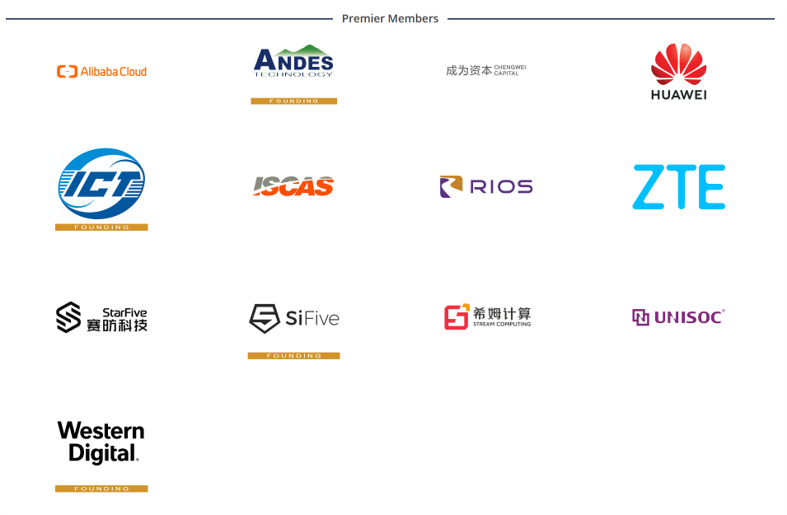
\includegraphics[width=1\textwidth]{RISC-V_Foundation_Members.png}
% 	\caption{RISC-V 基金会高级成员(评委老师说这张图要删掉)}
% 	\label{fig:figure1}
% \end{figure}

早期的RISC-V由于还在逐渐发展,大家对其仍然抱着观望的态度,主要还是用在一些功能比较简单的嵌入式芯片设计中,使用RISC-V设计的高性能处理器仍然较少,甚至早期还有人说RSIC-V不能用于开发高性能处理器。但是近几年来不断有国内的企业开始使用RISC-V设计高性能处理器,例如阿里巴巴的玄铁系列\cite{xuantie},而中科院计算所也研发了一款开源的RISC-V高性能处理器,命名为香山\cite{xiangshan},希望能够通过开源香山以及香山的开发流程和工具,探索高校设计制造处理器的可行性,并且希望能够搭建出一整套完善的集开发、调试、评估为一体的迭代流程。以此带动各路开发者的热情,打造一个良好的社区,促进处理器相关领域的发展。希望大家能够积极的参与到香山的开发与完善,也希望有人能够以香山为平台进行计算机体系结构的研究,未来更希望能有企业使用香山芯片制造出自己的产品。而本文的研究就是在香山处理器的开发平台上进行的,在香山第一版架构雁栖湖的基础上进行重构和迭代,设计实现了香山第二版架构南湖。目前香山第一版架构已经流片成功,第二版架构已经完成了时序调优,后端测试无误后即将送往流片。

在一个高性能处理器架构里,分支预测是必不可少的一个部件。由于分支指令会导致处理器的指令流水线出现中断,因此一个高效的分支预测部件能够尽可能地减少流水线中断的情况,极大提升处理器的整体性能,同时也能够降低流水线执行无效指令产生的额外功耗。由于现代的处理器都在往更高的频率,更深的流水线发展,以期待获得更高的性能。但同时更高的频率也限制了每个流水级间逻辑门级的数量,更深的流水线则造成了更大的分支误预测惩罚。并且处理器执行的程序指令数量也变得越来越多。在这种前提下,导致分支预测性能即使是一点点小小的提升,都能够对处理器的整体性能带来不可忽视的改变。因此高性能处理器的不断发展对分支预测的设计带来了更大的挑战\cite{bpu-overview},如何在满足频率要求的前提下实现预测算法,并且保证较高的分支预测准确率,是所有工程师和学者们都不断在研究推进的课题,各种各样的预测算法不断被提出,改进。

香山处理器第一版的分支预测参考了加州大学伯克利分校开发的一款开源RISC-V处理器BOOM (The Berkeley Out-of-Order Machine) 的分支预测设计\cite{boom-spec}。该分支预测设计有4级流水,使用混合预测器,以TAGE预测器作为主要的预测器。之所以选择以BOOM作为参考,首先是由于它作为一款开源的高性能处理器,可以直接接触到源代码,方便学习理解,且BOOM有过一次成功流片的经验,在业内的认可度也比较高。其次由于设计代码与香山开发使用的是相同的Chisel语言\cite{chisel},因此BOOM能够为香山带来许多的参考思路。例如香山在开发中有借鉴BOOM的参数管理机制,以及一些使用了Chisel语言特性的设计。

在讨论先进的分支预测算法和设计时,现有的论文大多基于模拟器来建模研究,没有考虑到具体的硬件实现,以及针对高频的优化。在真实的物理设计中,由于硬件特性和时序要求,相对于论文中的设计,在某些地方可能需要做出针对性的修改和优化,才能够将其真正的在硬件上实现。除了BOOM以外,有先进分支预测架构的开源设计也是寥寥无几,只能够通过公司的相关产品介绍和论文中窥到一些细节。因此本文以国内开源RISC-V高性能处理器香山为研究平台,在其第一版架构的基础上对分支预测进行了重构和优化,使其能够达到更高的性能和频率。同时,所有的设计代码都是开源的,能够给RISC-V社区中的开发者们提供借鉴和启发。

\section{国内外研究现状}


\subsection{RISC-V发展现状}
RISC-V是加州大学伯克利分校在2010年首次发布的一个开源指令集架构,2015年成立RISC-V基金会,而国内在2018年也成立了中国RISC-V产业联盟 (CRVIC)。这是一个年轻的指令集架构,它是吸收了大量已有指令集,如x86,ARM,MIPS等指令集的设计经验,弥补了它们的不足,做出大量的改进后产生的,并且为了给体系结构领域注入新的活力,RISC-V拥抱开源,使用RISC-V无需支付任何费用,让全世界的开发者能够不受成本政治等边缘因素的影响,全新的投入到RISC-V的设计与开发中来。

除了开源免费以外,RISC-V作为一个全新的指令集架构,不需要考虑历史兼容性的问题,这也使得它能够更加精简,门槛更低,相比于x86和ARM动辄几千页的手册,RISC-V的手册只有寥寥几百页,学习门槛大大降低,开发者们能够在更短的时间内掌握RISC-V设计的基础。并且RISC-V考虑到针对不同领域的不同需求,使用了模块化设计,除了基本的几十条指令以外,其他的都被模块化为一个个的扩展,开发者可以根据具体应用的需要,实现不同的扩展,而不用将所有的指令都实现,这使得RISC-V非常的多变与灵活,开发者也可以在RISC-V的基础上实现自定义指令,来满足产品的功能需求。

由于多种因素,RISC-V一出世就受到了工业界和学术界的关注与肯定。在经过一段时间的发展与完善后,大家都开始尝试以RISC-V为基础进行研究与设计。大量的研究成果也不断发布,最具代表性的就是加州大学伯克利分校的Rocket\cite{rocket}和BOOM两款开源的处理器设计,其中BOOM作为开源高性能处理器的代表,更是在大量的论文中作为研究平台和对比对象。而国内也有大量的成果,例如在阿里巴巴2021年9月10日正式开源的玄铁910,就是一款使用RISC-V指令集的处理器。此外国内还有很多公司都有相关的产品,如华米科技的黄山1号、紫光展锐的春藤系列,以及兆易创新的GD32VF103等。随着越来越多企业的加入,RISC-V也在不断地完善和发展自己的生态,

\subsection{分支预测发展现状}

分支预测器也有着不同的类型,首先是最简单的静态分支预测,静态分支预测通过一些静态的信息来进行预测,而不会考虑指令动态执行时的不同情况,例如可以将所有的分支都预测为跳转或不跳转\cite{branch-98},或者将向后跳转的分支预测为跳转,将向前的分支预测为不跳转。与之对应的就是更复杂,更准确的动态分支预测。动态分支预测能够通过收集程序运行时指令的动态信息来进行训练,学习到分支指令跳转的模式,根据不同情况给出预测,这样能够达到更加高的准确率,当然同时就对预测算法与硬件实现提出了更高的要求。由于更高的预测准确率,因此大部分处理器还是使用动态预测器为主。也有一些预测器不作为主要的预测器,而是作为在某个特定场景下使用的辅助预测器,比如循环预测器用于学习嵌套循环中循环指令的迭代次数,还有返回地址栈 (Return Address Stack, RAS),专门用于预测函数调用和返回指令的跳转地址。

分支预测器按照功能也分为两类,一种是方向预测器,比如TAGE预测器,这类预测器在预测时只会给出指令是否跳转的预测,而不会给出指令的跳转地址。另一种就是地址预测器,比如间接跳转预测器,用于在预测间接跳转分支时给出跳转地址。最常见的地址预测器就是各种各样的BTB (Branch Target Buffer)了,用于在还没有得到指令预译码信息时给出分支指令的跳转地址,并且有着许多不同的设计和实现。

此外分支预测器也可以按照使用的分支历史分为局部历史预测器和全局历史预测器。程序执行时可以记录所有分支指令的跳转历史,用1表示跳转,0表示不跳转,通过这些历史对预测器进行训练,找到特定的模式来为后续的分支指令做预测。局部历史预测器倾向于使用部分的分支历史来做预测,例如循环预测器只会寻找可能是循环跳转指令的分支。而全局历史预测器会倾向于使用所有的分支历史或某种全局分支历史的哈希,例如TAGE预测器。两种类型的预测器都各有优劣,因此将它们混合使用往往可以更好的覆盖不同的分支指令。

在现在的主流高性能处理器中一般使用的都是混合分支预测器,即同时包含多种预测器,在不同的情况下分别选择使用不同预测器的预测结果,以达到覆盖更多类型分支,以及满足硬件设计要求的目的。通常会有一个简单的预测器,它的预测速度很快,一个周期就能够给出预测结果,用于保证分支预测流水线不会中断,然后还有一个主要的预测器,可能需要2-3个周期才会出预测结果。最终会根据不同情况,选择最合适的预测器的预测结果送往取指。

\subsection{现有处理器的分支预测设计}

\begin{itemize}[listparindent=2em]
	\item BOOM (the Berkeley Out-
    of-Order Machine)\cite{boom-spec, sonic-boom}使用了耦合的前端设计,总共有4级取指流水级,其中在F1,F2,F3会分别得到不同预测器的预测结果,并且当后面的预测结果和前面不同时,需要纠正前面的错误预测。在F1使用Micro BTB进行预测,F2使用BIM和BTB进行预测,F3使用TAGE进行预测。
    
    此外BOOM还实现了循环预测器和RAS (Return Address Stack),循环预测器用于在某些嵌套循环指令中,预测循环体的循环跳转指令。RAS用于预测call和return指令。

    \begin{figure}[htb]
        \centering
        \setlength\tabcolsep{3pt}  % 同一行中的图片间隔
        \vspace{5pt} % 图片上部的空白,如果太小的话,图片顶部会与正文内容十分接近
        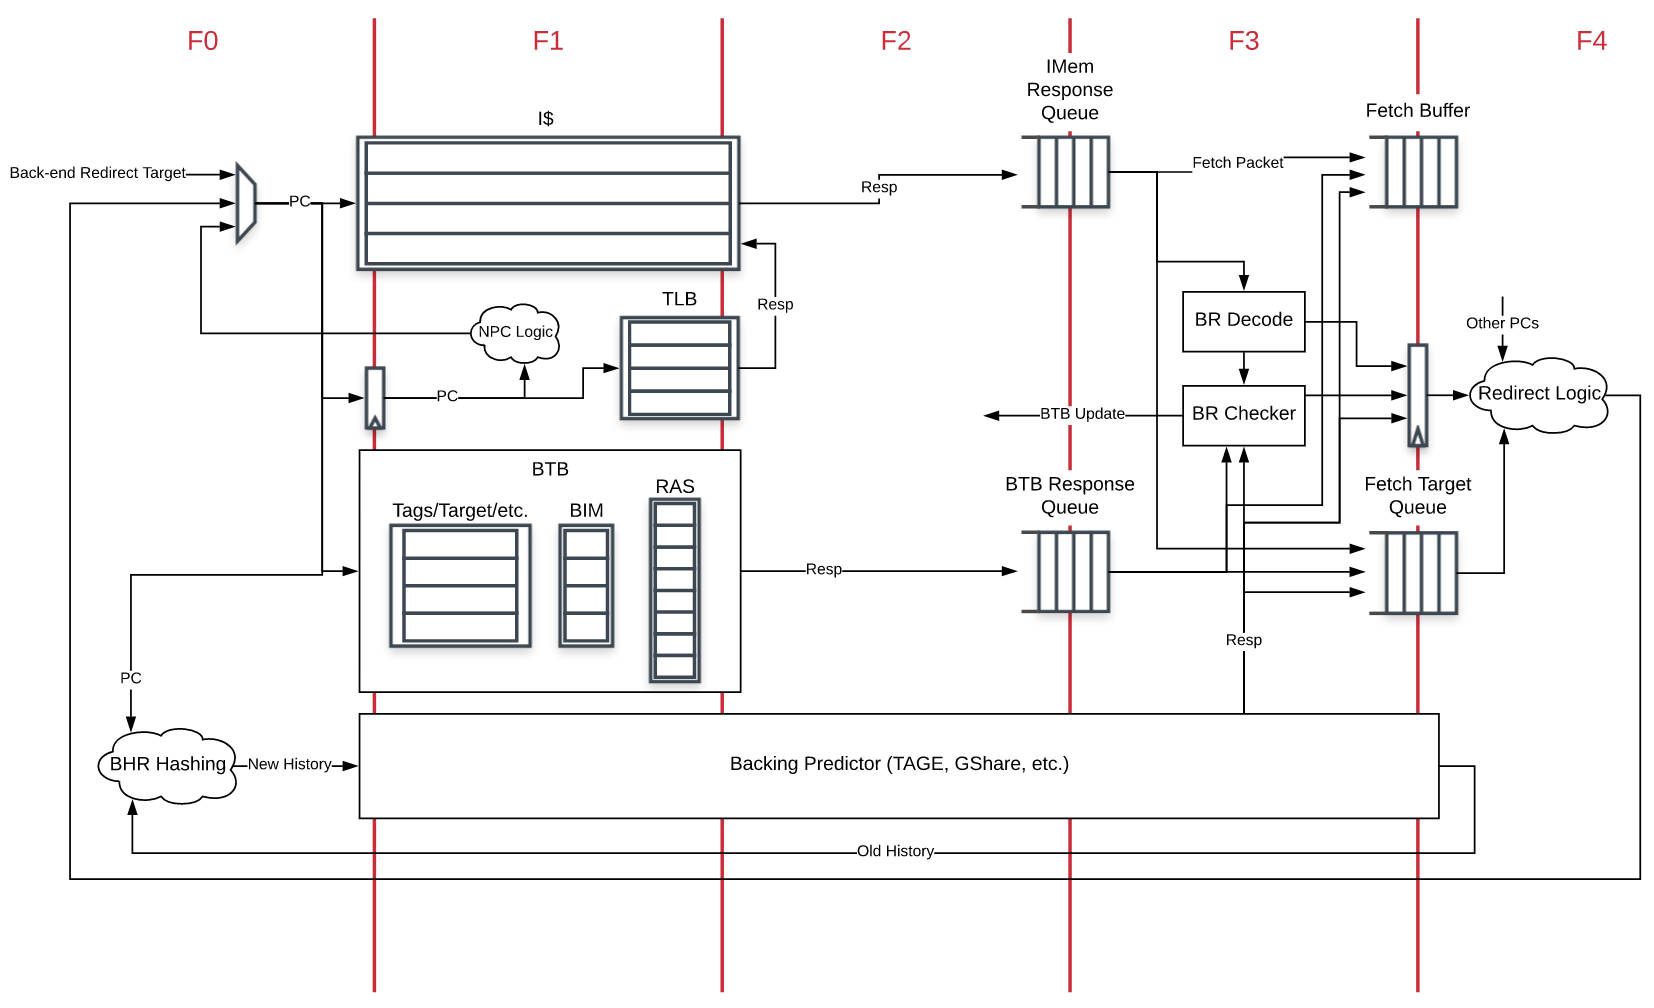
\includegraphics[width=1\textwidth]{boom-frontend.jpg}
        \caption{BOOM前端架构图\cite{boom-frontend}}
        \label{fig:figure11}
    \end{figure}

	\item 玄铁910\cite{xuantie}使用了耦合的前端设计,即取指单元和分支预测流水级是耦合的,采用了两级的混合预测器的结构设计。在IP级就可以得到预译码信息,可以直接解析出一些直接跳转指令的跳转目标地址。

    玄铁910使用BHT(branch target table)来存储分支跳转历史,使用了一种类似BI-MODE\cite{bi-mode}机制的方向预测器。在IF级有一个16项全相联的L0 BTB (Branch Target Buffer),在IP级有一个1K项组相联的L1 BTB。使用覆盖预测,当IP级的预测结果与IF级不同时需要将之前的预测结果纠正回来。这种设计和香山的第一版是类似的。

    此外玄铁910还有支持12级函数调用嵌套的RAS;循环加速器 (Loop Buffer),用于将循环体中的指令缓存下来,关闭指令缓存来节省功耗;间接跳转预测器,用于预测间接跳转指令的目标地址。

    \item 龙芯GS464E\cite{loongson}前端依然是耦合的设计,总共有3个流水级,也是多种预测器混合使用,在每周期最多可以处理4条分支指令。龙芯GS464E中实现了一个分支目标缓冲器 (BrBTB),功能类似于BOOM的Micro BTB,都是为了在更准确的预测器结果出来之前,做一个简单的预测,尽可能提高流水线的连续性,不同之处在于龙芯GS464E的BrBTB是放在IF4级流水级的。除了BrBTB外,还有更加准确的预测器,实现了一套组合分支历史表 (BHTs),包含3张16K项的表,分别是全局转移历史表 (global branch history table, GBHT),局部转移历史表 (local branch history table, LBHT)和全局选择历史表 (global branch select table, GSEL)。此外还有RAS,和用于预测间接跳转指令的跳转目标缓存器 (jump branch target address cache, JBTAC),和玄铁910类似的Loop Buffer。
    
    
    \begin{figure}[htb]
        \centering
        \setlength\tabcolsep{3pt}  % 同一行中的图片间隔
        \vspace{5pt} % 图片上部的空白,如果太小的话,图片顶部会与正文内容十分接近
        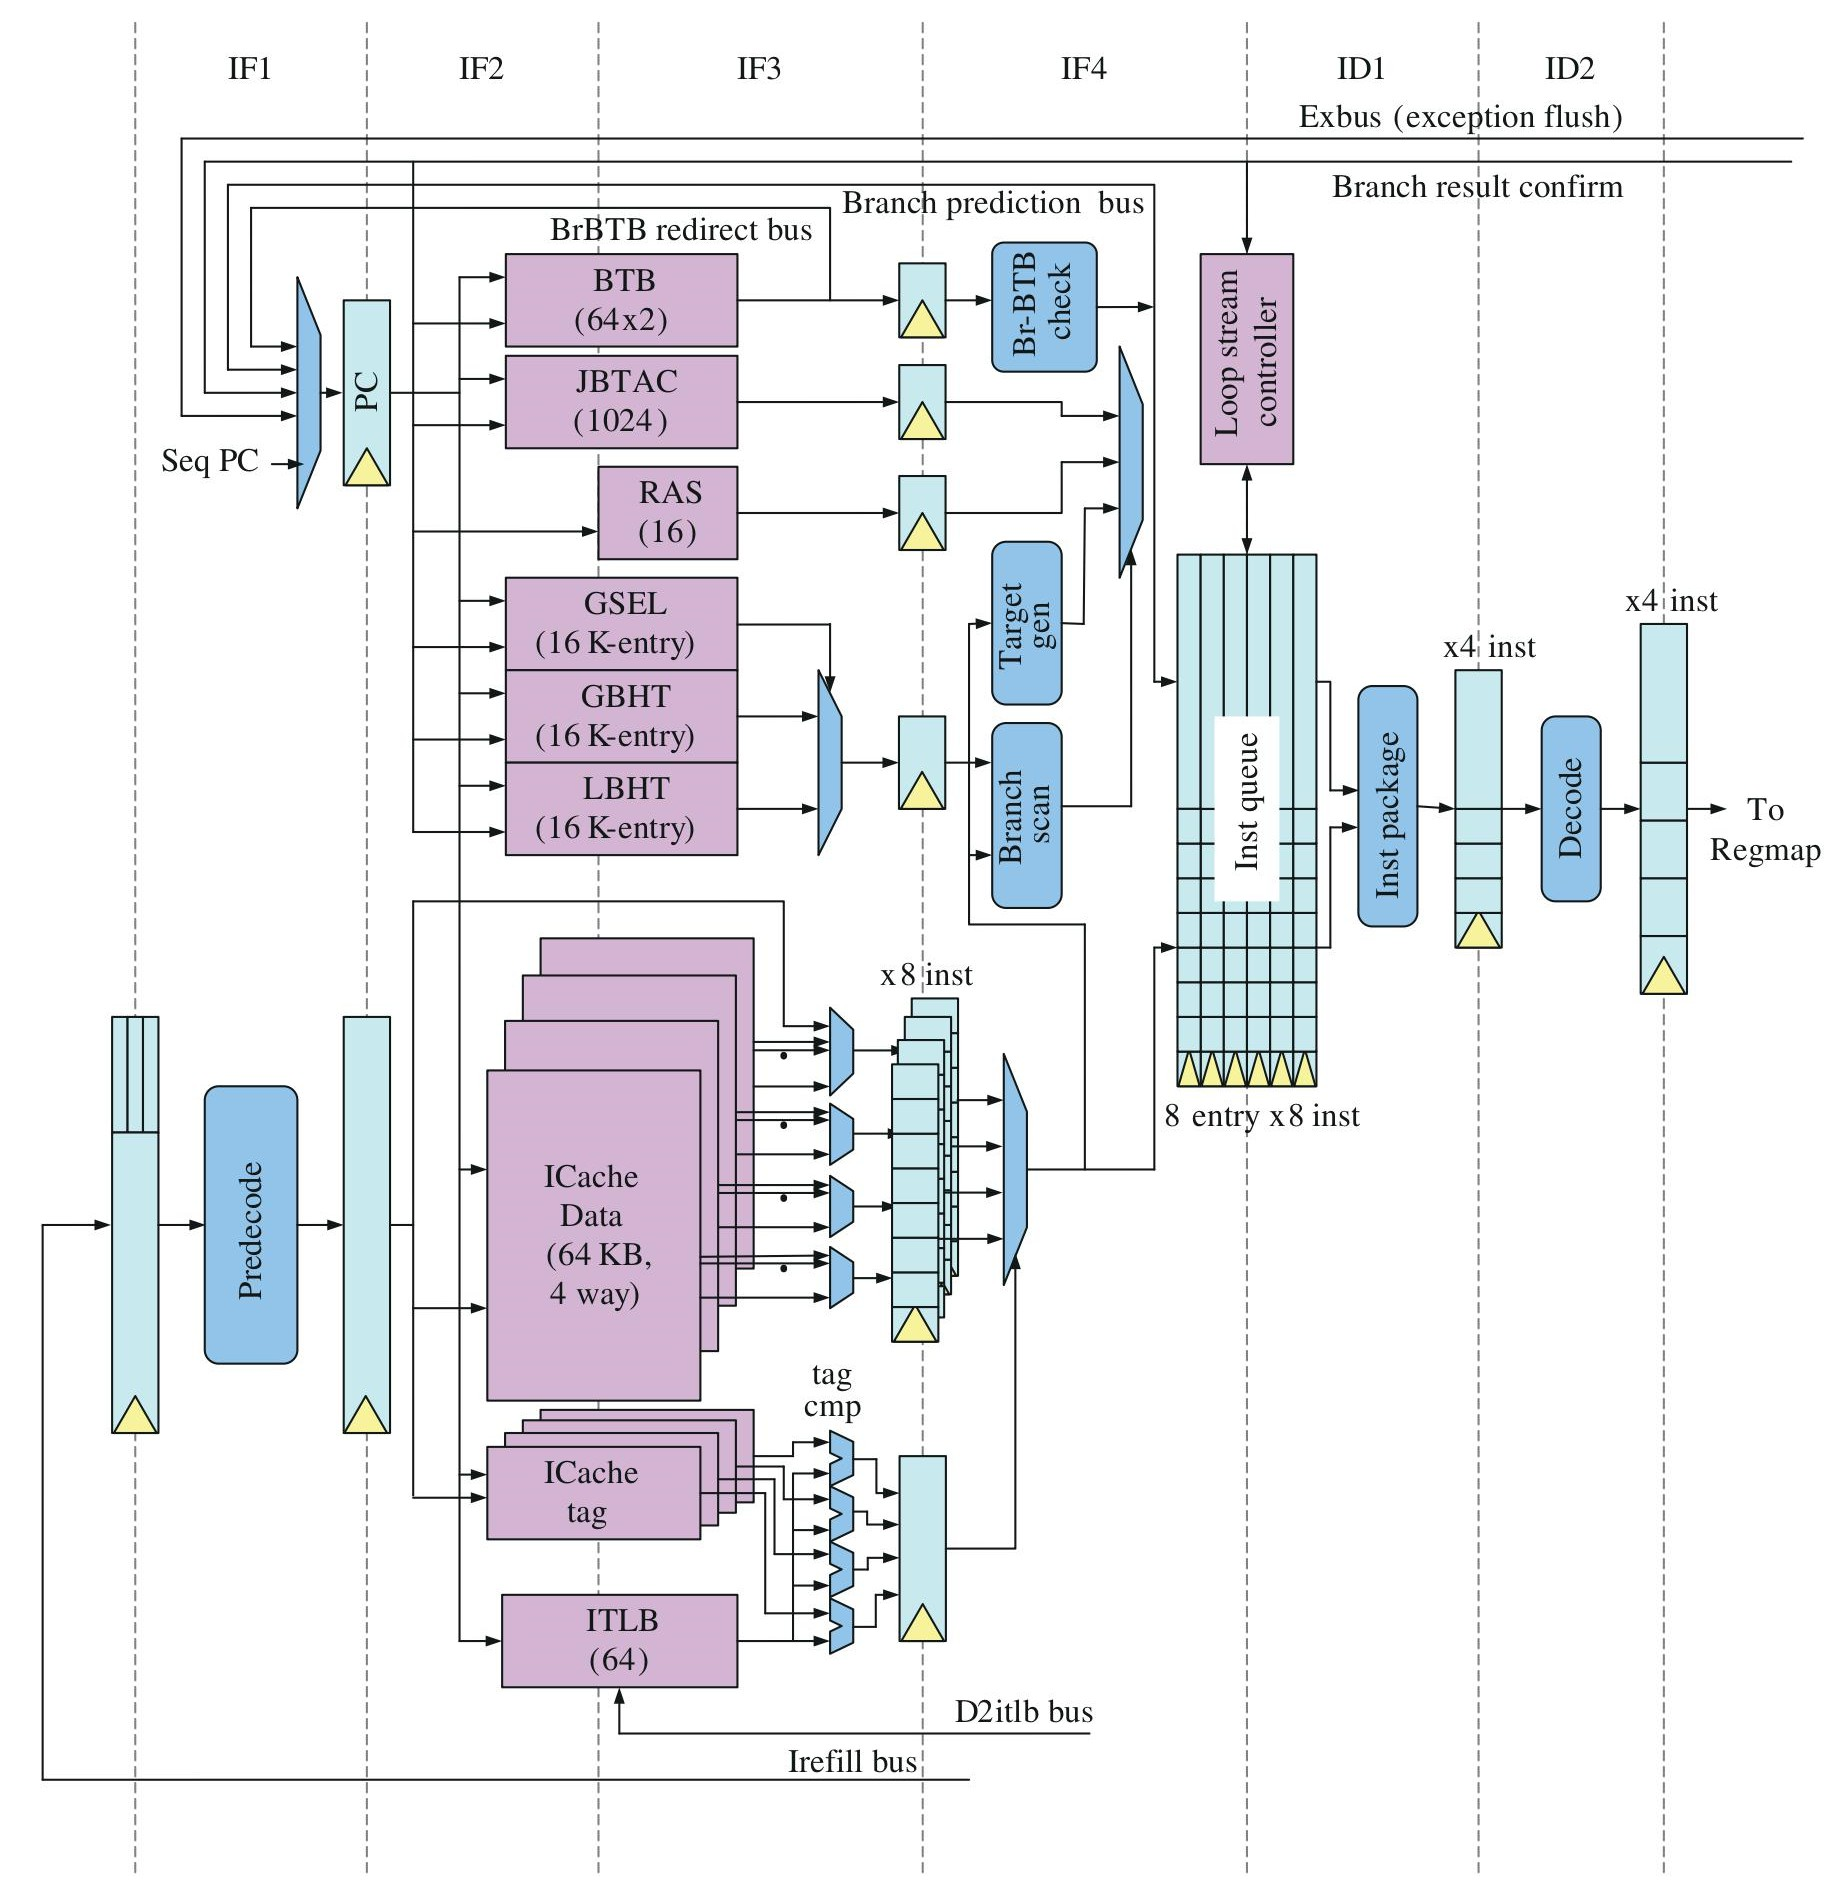
\includegraphics[width=1\textwidth]{loongson-frontend.jpg}
        \caption{龙芯GS464E前端架构图\cite{loongson}}
        \label{fig:figure12}
    \end{figure}
    
    \item Samsung Exynos\cite{samsung-exynos}使用了解耦的前端,主要的分支预测器使用的是改进的Scaled Hashed Perceptron (SHP)算法\cite{perceptrons,neural-branch,optimized-neural,strided-perceptron,merging-perceptron},同样是混合预测,有一个小而快的micro-BTB (μBTB) 和一个本地历史散列感知器 (LHP),主要的分支预测器是main-BTB (mBTB)和SHP。还实现了RAS,Level-2 BTB (L2BTB) 以及virtual address-based BTB (vBTB)。间接跳转预测器使用的是virtual program counter (VPC)\cite{vpc} 预测器。
\end{itemize}

从以上几个处理器的分支预测设计可以看出,目前混合预测的设计是主流方案,一般倾向于一个小而快的预测器搭配上一个准但是慢的主要预测器,再加上一些针对特定指令的预测器,例如RAS和间接跳转预测器等。虽然在以上几个处理器设计中只有Samsung Exynos是解耦前端,但是根据与其他设计团队的交流来看,解耦前端确实是目前主流商用处理器都在使用的一个方案。

% \subsection{引用参考文献}
% 在references.bib中添加参考文献对应的bibtex,使用$\backslash$cite\{\}引用论文的id,如引用参考文献\cite{barnes2009patchmatch}。

% \subsection{插入图片}
% 如图\ref{fig:figure1}所示,在文章中插入图片。使用$\backslash$begin\{figure\}插入图片,支持的格式有jpg、png、eps与pdf等,本例使用$\backslash$begin\{tabular\}插入三幅图像(一行三列),如果只插入一副图像则不需使用$\backslash$begin\{tabular\}。

% \begin{figure}[htb]
% 	\centering
% 	\setlength\tabcolsep{3pt}  % 同一行中的图片间隔
% 	\vspace{5pt} % 图片上部的空白,如果太小的话,图片顶部会与正文内容十分接近
% 	\begin{tabular}{ccc}
% 		\includegraphics[width=0.32\textwidth]{baboon.jpg} &
% 		\includegraphics[width=0.32\textwidth]{lena.jpg} &
% 		\includegraphics[width=0.32\textwidth]{parrot.jpg} \\
% 		(a) 图1 & (b) 图2 & (c) 图3 \\[1ex]
% 	\end{tabular}
% 	\caption{图片示例}
% 	\label{fig:figure1}
% \end{figure}

% \subsection{插入公式}
% 如公式\eqref{eq:equation1}所示,为公式示例:
% \begin{equation}
% 	c = a + b
% 	\label{eq:equation1}
% \end{equation}

% \subsection{插入表格}

% 如表格\ref{tb:table1}所示,为表格示例。可以通过"https://www.tablesgenerator.com/"以用户界面形式创建表格,并将表格转化为latex代码。

% \begin{table}[]
% 	\caption{表格标题}
% 	\label{tb:table1}
% 	\centering
% 	\begin{tabular}{|c|c|c|}
% 		\hline
% 		a   & b   & c   \\ \hline
% 		1.1 & 1.2 & 1.3 \\ \hline
% 		1.4 & 1.5 & 1.6 \\ \hline
% 	\end{tabular}
% \end{table}

\section{本文思路及研究方法}

本文首先介绍了开源RISC-V高性能处理器在国内的研究意义,以及为什么选择使用RISC-V来设计处理器的原因,之后简单介绍了分支预测的发展现状,不同类型的预测器以及它们各自的特点。并对香山超标量乱序处理器分支预测的基本结构和各个预测器的功能和设计思路做了介绍。之后进一步介绍了分支预测部件的整体架构,并在此基础上从性能和频率两个方面对其进行了优化。

\begin{itemize}
	\item 性能方面。通过将第一版架构的前端分支预测和取指部分解耦,减少了前端流水线由于分支预测和取指单元共用流水级导致的不必要的阻塞。其中主要介绍了FTQ (Fetch Target Queue)这个主要模块的功能和行为逻辑。
	\item 频率方面。为了减少分支预测整体的预测宽度,将整个分支预测的基本单位由单条分支改为了Fetch Block,通过定义约束来限制每次取指的block中分支指令的上限。主要介绍FTB (Fetch Target Buffer)这个主要模块的功能和行为逻辑。
\end{itemize}

介绍完相关的优化之后,我们使用Design Compiler对整个处理器架构进行了时序评估,并使用Verilator对整体设计进行行为级仿真,运行SPEC2006测试程序,通过分析相关的性能数据用于评估其改进结果。

\section{论文结构}

本文分为以下几个章节,内容安排如下:

第一章的主要内容是介绍了本课题的研究背景和意义,讨论了一些国内外的研究现状,分支预测器的分类。简单介绍了香山处理器的整体架构,并对本文内容做了规划。

第二章的主要内容是介绍分支预测架构流水级,以及各个流水级中预测器的分布,然后介绍各个预测器的功能及其设计实现细节。

第三章的主要内容是介绍以FTB为主的限制分支预测宽度的分支预测改进策略,并给出了FTB的详细数据结构设计,以及更新管理策略。

第四章的主要内容是提出以FTQ为主的实现解耦前端取指单元的设计,详细介绍了FTQ与分支预测、取指单元、后端执行单元交互的各种功能和逻辑。

% 第五章的主要内容是介绍了针对改进分支预测性能做过的部分尝试及其细节

第五章的主要内容是介绍开发和评估测试设计所用到的环境,以及相关的评估指标,统计结果及其分析。

第六章的主要内容是对本文工作的一个总结,并指出目前仍然存在的一些问题,提出了一些已知的改进方向,对之后的工作做出了展望。

